\documentclass[11pt]{article}

\usepackage[T1]{fontenc}
\usepackage[utf8]{inputenc}

\usepackage[ruled,vlined,linesnumbered]{algorithm2e}
\SetKwInput{KwData}{Input}
\SetKwInput{KwResult}{Result}

\PassOptionsToPackage{hyphens}{url}
\usepackage[
colorlinks=true,linkcolor=blue,urlcolor=blue,citecolor=blue,bookmarks=true,
bookmarksopenlevel=2]{hyperref}
\usepackage{amsmath,amssymb,amsthm,textcomp}

\usepackage{cleveref}

\usepackage{minted}
\usepackage{tikz}
\definecolor{gray}{rgb}{0.85,0.85,0.85}
\setminted[bash]{bgcolor=gray}
\setminted[python]{breaklines}

\usepackage{graphicx}

\usepackage{geometry}
\geometry{%total={210mm,297mm},
left=25mm,right=25mm,%
bindingoffset=0mm, top=20mm,bottom=20mm}

\setlength\parindent{0pt}
\setlength{\parskip}{1mm}
\setcounter{section}{-1}

\sloppy

\begin{document}

\title{Student Tasks}
\author{Wolfgang Hönig\footnote{Now at California Institute of Technology}, Jiaoyang Li, Sven Koenig --- University of Southern California}
\date{Model AI Assignments 2020: A Project on Multi-Agent Path Finding (MAPF)}

\maketitle

In this project, you will learn about Multi-Agent Path Finding (MAPF) and implement a single-agent solver, namely space-time A*, and parts of three MAPF solvers, namely prioritized planning, Conflict-Based Search (CBS), and CBS with disjoint splitting.

\section{Task 0: Preparing for the Project}

\subsection{Installing Python 3}

This project requires a Python 3 installation with the \texttt{numpy} and \texttt{matplotlib} packages. On Ubuntu Linux, download python by using:

\begin{minted}{bash}
sudo apt install python3 python3-numpy python3-matplotlib
\end{minted}

On Mac OS X, download Anaconda 2019.03 with Python 3.7 from \url{https://www.anaconda.com/distribution/#download-section} and follow the installer. You can verify your installation by using:

\begin{minted}{bash}
python3 --version
\end{minted}

On Windows, download Anaconda 2019.03 with Python 3.7 from \url{https://www.anaconda.com/distribution/#download-section}. 

\textcolor{red}{On Ubuntu Linux and Mac OS X, use \texttt{python3} to run python. On Windows, use \texttt{python} instead.}

You can use a plain text editor for the project. If you would like to use an IDE, we recommend that you download PyCharm from \url{https://www.jetbrains.com/pycharm/}. The free community edition suffices fully, but you can get the professional edition for free as well, see \url{https://www.jetbrains.com/student/} for details.

\subsection{Installing the MAPF Software}

Download the archive with the provided MAPF software and extract it on your computer.

\subsection{Learning about MAPF}

Read the provided textbook-style overview of MAPF.

\subsection{Understanding Independent Planning}

Execute the independent MAPF solver by using:

\begin{minted}{bash}
  python run_experiments.py --instance instances/exp0.txt --solver Independent
\end{minted}

If you are successful, you should see an animation:

\begin{center}
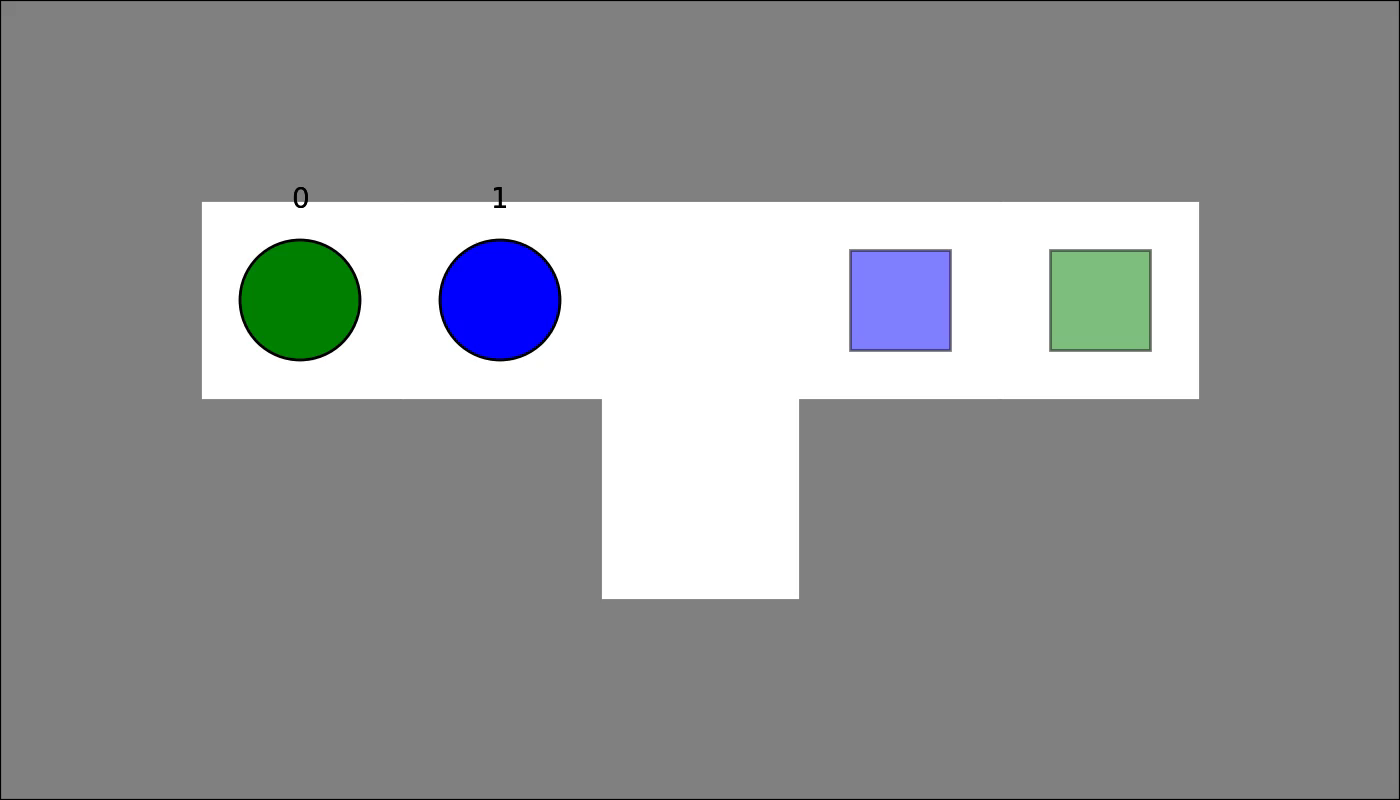
\includegraphics[width=0.3\textwidth]{images/exp1_1.png}
\hfill
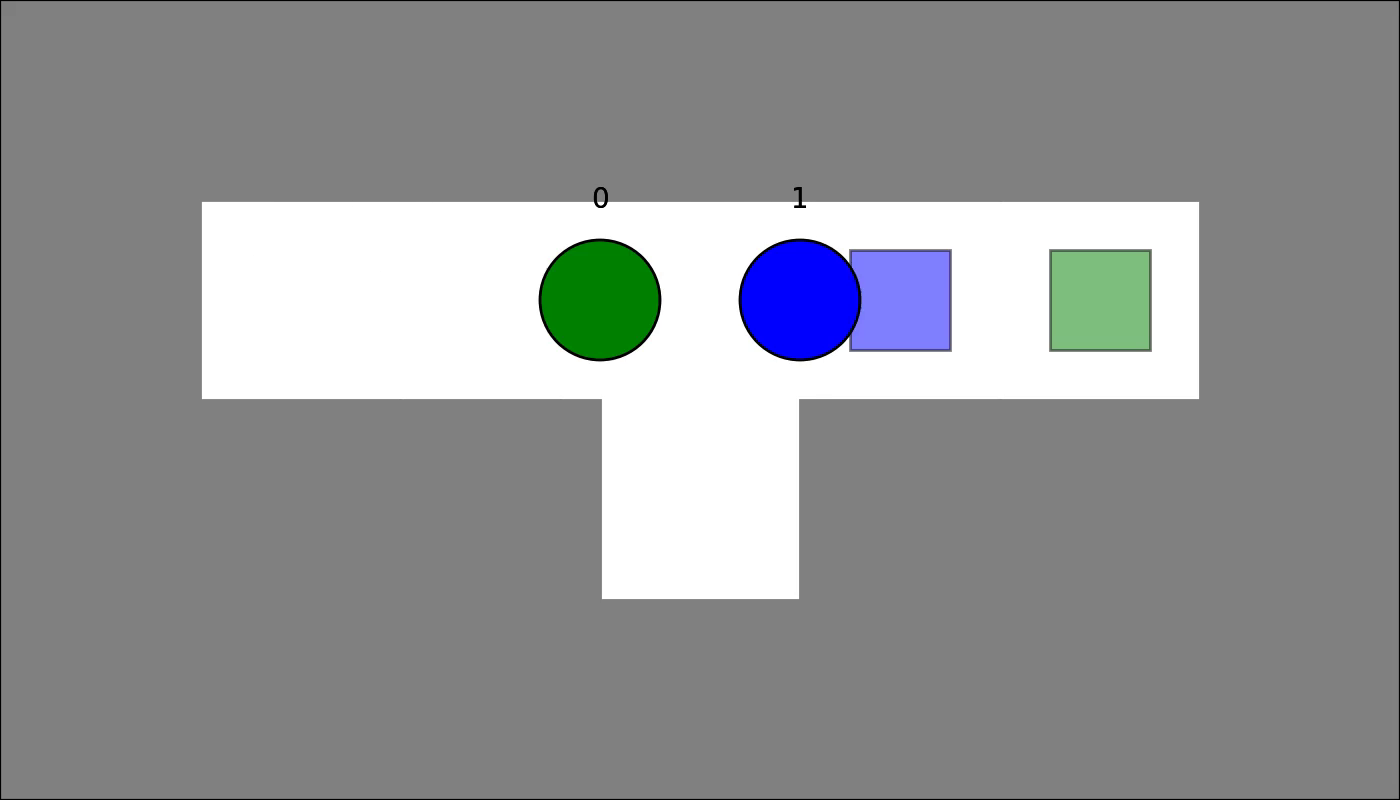
\includegraphics[width=0.3\textwidth]{images/exp1_2.png}
\hfill
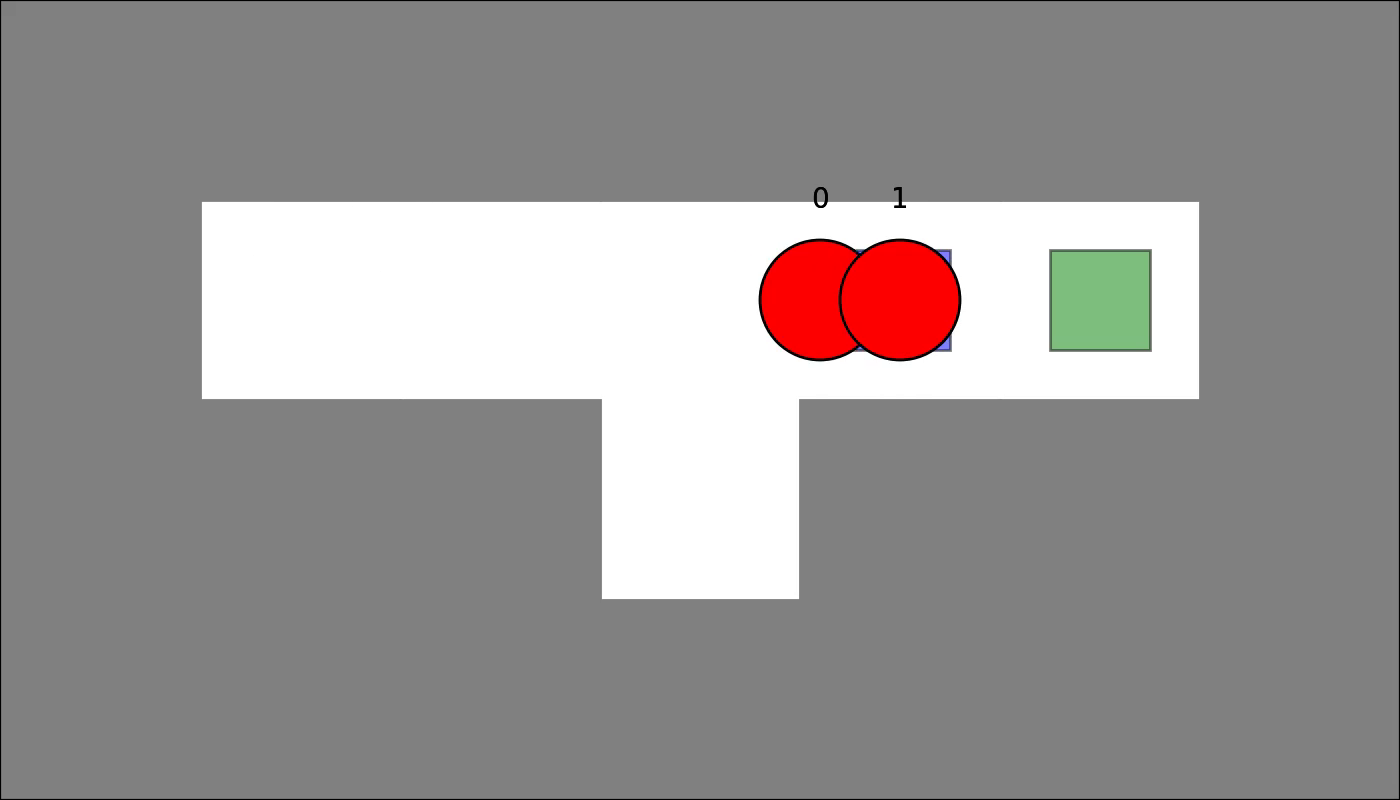
\includegraphics[width=0.3\textwidth]{images/exp1_3.png}
\end{center}

The independent MAPF solver plans for all agents independently. Their paths do not collide with the environment but are allowed to collide with the paths of the other agents. Thus, there is a collision when the blue agent 1 stays at its goal cell while the green agent 0 moves on top of it. In your animation, both agents turn red when this happens, and a warning is printed on the terminal notifying you about the details of the collision.

Try to understand the independent MAPF solver in \texttt{independent.py}. The first part defines the class \mintinline{python}{IndependentSolver} and its constructor:

\begin{minted}{python}
class IndependentSolver(object):
    def __init__(self, my_map, starts, goals):
        # some parts are omitted here for brevity
        # compute heuristic values for the A* search
        self.heuristics = []
        for goal in self.goals:
            self.heuristics.append(compute_heuristics(my_map, goal))
\end{minted}

The function \mintinline{python}{compute_heuristics} receives as input the representation of the environment and the goal cell of the agent and computes a look-up table with heuristic values (or, synonymously, h-values) for the A* search that finds a path for the agent, by executing a Dijkstra search starting at the goal cell.

The second part performs one A* search per agent:

\begin{minted}{python}
    def find_solution(self):
         for i in range(self.num_of_agents):  # Find path for each agent
            path = a_star(self.my_map, self.starts[i], self.goals[i], self.heuristics[i], i, [])
            if path is None:
                raise BaseException('No solutions')
            result.append(path)
        return result
\end{minted}

The function \mintinline{python}{a_star} receives as input the representation of the environment, the start cell of the agent, the goal cell of the agent, the heuristic values computed in the constructor, the unique agent id of the agent, and a list of constraints and performs an A* search to find a path for the agent. The independent MAPF solver does not use constraints. 

\section{Task 1: Implementing Space-Time A*}

You now change the single agent solver to perform a space-time A* search that searches in cell-time space and returns a shortest path that satisfies a given set of constraints. Such constraints are essential for MAPF solvers such as prioritized planning and CBS.

\subsection{Searching in the Space-Time Domain}

The existing A* search in the function \mintinline{python}{a_star} in \texttt{single\_agent\_planner.py} only searches over cells. Since we want to support temporal constraints, we also need to search over time steps. Use the following steps to change the search dimension:

\begin{enumerate}
    \item Your variables \mintinline{python}{root} and \mintinline{python}{child} are dictionaries with various key/value pairs such as the g-value, h-value, and cell. Add a new key/value pair for the time step. The time step of the root node is zero. The time step of each node is one larger than the one of its parent node.
    \item The variable \mintinline{python}{closed_list} contains the processed (that is, expanded) nodes. Currently, this is a dictionary indexed by cells. Use tuples of (cell, time step) instead.
    \item When generating child nodes, do not forget to add a child node where the agent waits in its current cell instead of moving to a neighboring cell.
\end{enumerate}

You can test your code by using:

\begin{minted}{bash}
  python run_experiments.py --instance instances/exp1.txt --solver Independent
\end{minted}

and should observe identical behavior.

\subsection{Handling Vertex Constraints}

We first consider (negative) vertex constraints, that prohibit a given agent from being in a given cell at a given time step.

Each constraint is a Python dictionary. The following code creates a (negative) vertex constraint that prohibits agent 2 from occupying cell $(3,4)$ at time step 5:

\begin{minted}{python}
{'agent': 2,
 'loc': [(3,4)],
 'timestep': 5}
\end{minted}

In order to add support for constraints, change the code to check whether the new node satisfies the constraints passed to the \mintinline{python}{a_star} function and prune it if it does not.

An efficient way to check for constraint violations is to create, in a pre-processing step, a constraint table, which indexes the constraints by their time steps. At runtime, a lookup in the table is used to verify whether a constraint is violated. Example function headers for the functions \mintinline{python}{build_constraint_table} and \mintinline{python}{is_constrained} are already provided. You can call \mintinline{python}{build_constraint_table} before generating the root node in the \mintinline{python}{a_star} function.

You can test your code by adding a constraint in \texttt{prioritized.py} that prohibits agent 0 from being at its goal cell $(1,5)$ at time step 4 and then using:

\begin{minted}{bash}
  python run_experiments.py --instance instances/exp1.txt --solver Prioritized
\end{minted}

Agent 0 should wait for one time step (but when and where it waits depends on the tie-breaking).

\subsection{Adding Edge Constraints}

We now consider (negative) edge constraints, that prohibit a given agent from moving from a given cell to another given cell at a given time step.

The following code creates a (negative) edge constraint that prohibits agent 2 from moving from cell $(1,1)$ to cell $(1,2)$ from time step 4 to time step 5:

\begin{minted}{python}
{'agent': 2,
 'loc': [(1,1), (1,2)],
 'timestep': 5}
\end{minted}

Implement constraint handling for edge constraints in the function \mintinline{python}{is_constrained}.

You can test your code by adding a constraint in \texttt{prioritized.py} that prohibits agent 1 from moving from its start cell $(1,2)$ to the neighboring cell $(1,3)$ from time step 0 to time step 1.

\subsection{Handling Goal Constraints}

Run your code with a constraint that prohibits agent 0 from being at its goal cell $(1,5)$ at time step 10. Where is agent 0 at time step 10 in your solution? To make the algorithm work properly, you might have to change the goal test condition. Explain what changes you made to the goal test condition. (The solution of both agents could have collisions.)
 
\subsection{Optional: Designing Constraints}

Design a set of constraints by hand that allows your algorithm to find collision-free paths with a minimal sum of path lengths. Run your code with the set of constraints. Document this set of constraints, the solution, and the sum of path lengths.

\section{Task 2: Implementing Prioritized Planning}

The independent MAPF solver finds paths for all agents, simultaneously or one after the other, that do not collide with the environment but are allowed to collide with the paths of the other agents. The prioritized MAPF solver finds paths for all agents, one after the other, that do not collide with the environment or the already planned paths of the other agents. To ensure that the path of an agent does not collide with the already planned paths of the other agents, the function \mintinline{python}{a_star} receives as input a list of (negative) constraints compiled from their paths.

\subsection{Adding Vertex Constraints}

Add code to \texttt{prioritized.py} that adds all necessary vertex constraints. You need two loops, namely one to iterate over the path of the current agent and one to add vertex constraints for all future agents (since constraints apply only to the specified agent). You can test your code by using:

\begin{minted}{bash}
  python run_experiments.py --instance instances/exp2_1.txt --solver Prioritized
\end{minted}

Now, the blue agent 2 does not stay at its goal cell when it reaches that cell for the first time:

\begin{center}
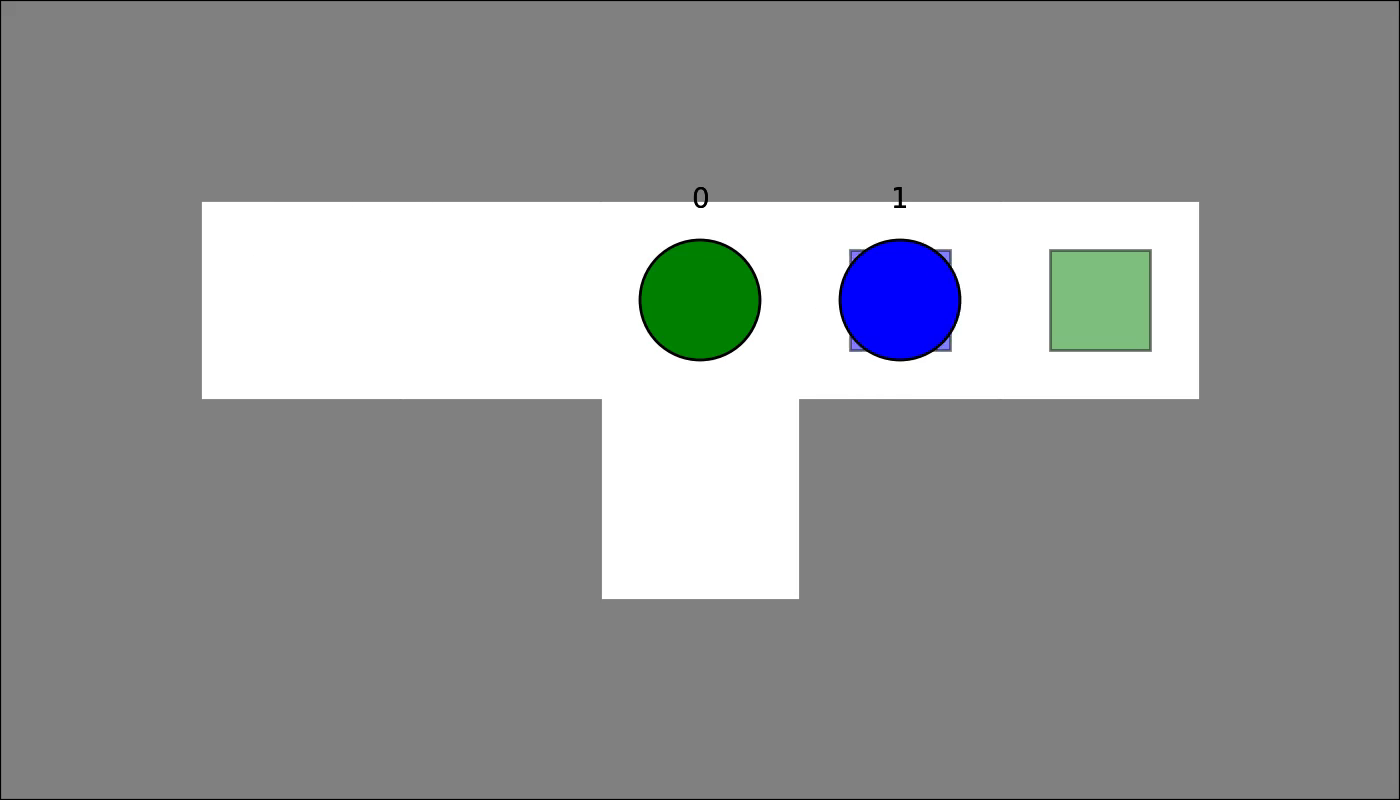
\includegraphics[width=0.3\textwidth]{images/exp1_seq1.png}
\hfill
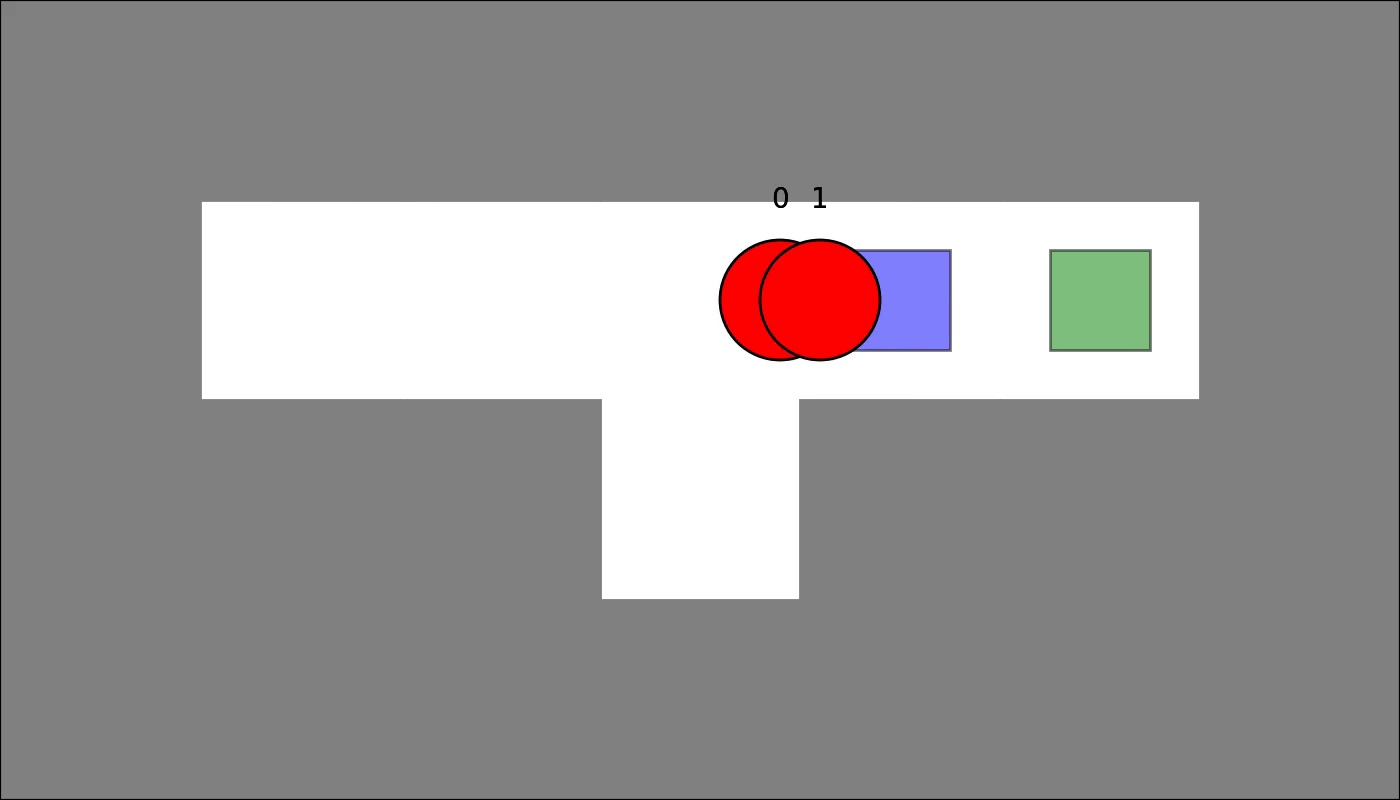
\includegraphics[width=0.3\textwidth]{images/exp1_seq2.png}
\hfill
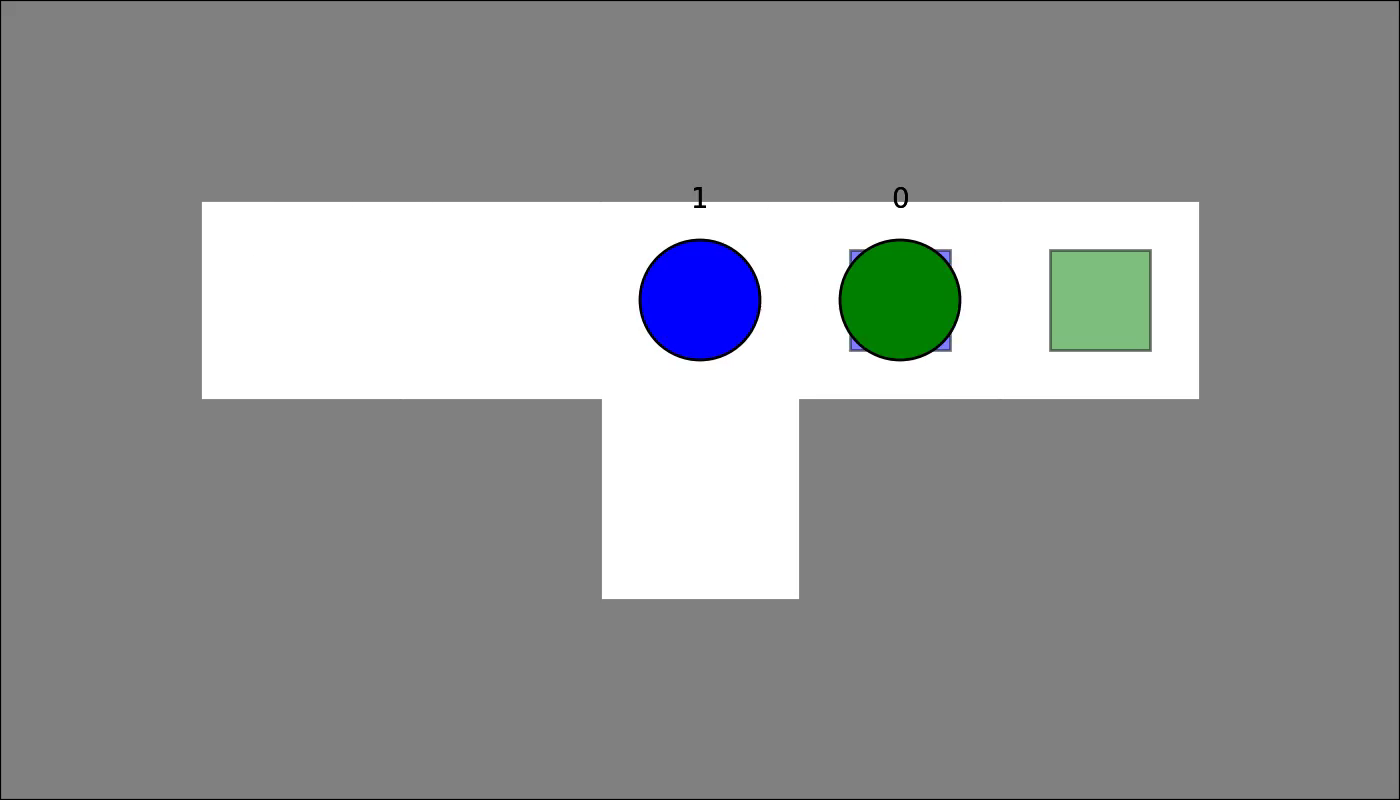
\includegraphics[width=0.3\textwidth]{images/exp1_seq3.png}
\end{center}

Unfortunately, there is still a collision because both agents move to the cell of the other agent at the same time step. We thus need to add (negative) edge constraints as well.

\subsection{Adding Edge Constraints}

Add code to \texttt{prioritized.py} that adds all necessary edge constraints, and test your code as before. There are no more collisions.

\subsection{Optional: Adding Additional Constraints \label{add}}

Your code does not prevent all collisions yet since agents can still move on top of other agents that have already reached their goal locations. You can verify this issue by using the MAPF instance \texttt{exp2\_2.txt} and assuming that agent 0 has the highest priority. 
You can address this issue by adding code that adds additional constraints that apply not only to the time step when agents reach their goal locations but also to all future time steps.

\subsection{Optional: Addressing Failures}

In the MAPF instance \texttt{exp2\_3.txt}, the priorities between agents 0 and 1 and are switched compared to \texttt{exp2\_2.txt}. Rerun the experiment on instance \texttt{exp2\_3.txt}. Did your solver terminate properly and report ``no solutions''? If not, describe what happened and change your code to address the issue. Hint: You can address this issue by limiting the time horizon of the search. The shortest path of an agent cannot be infinitely long. So you can calculate an upper bound on the path length for an agent based on the path lengths of all agents with higher priorities and the size of the environment.

\subsection{Optional: Showing that Prioritized Planning is Incomplete and Suboptimal}

Solve one or more of the following tasks either on paper or with the implementation of the prioritized MAPF solver after you have added the additional constraints from Section~\ref{add}:

\begin{itemize}

\item Design a MAPF instance for which prioritized planning does not find an (optimal or suboptimal) collision-free solution for a given ordering of the agents. 

\item Design a MAPF instance for which prioritized planning does not find an (optimal or suboptimal) collision-free solution, no matter which ordering of the agents it uses. 

\item Design a MAPF instance for which prioritized planning does not find an (optimal or suboptimal) collision-free solution for a given ordering of the agents even if an ordering of the agents exists for which prioritized planning finds an optimal collision-free solution. 

\item Design a MAPF instance for which prioritized planning finds a suboptimal (but not optimal) collision-free solution for a given ordering of the agents even if an ordering of the agents exists for which prioritized planning finds an optimal collision-free solution. 

\item Design a MAPF instance for which prioritized planning does not find an optimal collision-free solution, no matter which ordering of the agents it uses, even if a collision-free solution exists.

\end{itemize}

\section{Task 3: Implementing Conflict-Based Search (CBS)}

Conflict-Based Search (CBS) is slower than prioritized planning but complete and optimal.

\subsection{Detecting Collisions}

Write code that detects collisions (or, synonymously, conflicts) among agents, namely vertex collisions where two agents are in the same cell at the same time step and edge collisions where two agents move to the cell of the other agent at the same time step.

Add code to \texttt{cbs.py} that implements the two functions \mintinline{python}{detect_collision} and \mintinline{python}{detect_collisions}. You should use \mintinline{python}{get_location(path,t)} to obtain the cell of an agent at time step $t$. You can test your code by using:

\begin{minted}{bash}
  python run_experiments.py --instance instances/exp3_1.txt --solver CBS
\end{minted}

You receive output similar to

\begin{minted}{python}
  [{'a1': 0, 'a2': 1, 'loc': [(1, 4)], 'timestep': 3}]
\end{minted}

\subsection{Converting Collisions to Constraints}

The high level of CBS searches the constraint tree. Once it has chosen a node of the constraint tree for expansion and picked a collision of the paths of two agents in that node, it transforms this collision into two new (negative) constraints, one for each new child node of the chosen node. The first constraint prohibits the first agent from executing the colliding action, and the second constraint prohibits the second agent from executing the colliding action. For the vertex collision between agents 1 and 2 in cell $(1,4)$ at time step 3, the set of new vertex constraints is:

\begin{minted}{python}
[{'agent': 0, 'loc': [(1, 4)], 'timestep': 3},
 {'agent': 1, 'loc': [(1, 4)], 'timestep': 3}]
\end{minted}

Add code to \texttt{cbs.py} that implements the function \mintinline{python}{standard_splitting} and test your code as above. Hint: You need to reverse the direction of the edge for the second agent to obtain the second edge constraint for an edge collision.

\subsection{Implementing the High-Level Search}

\SetInd{0.5em}{0.5em}
\begin{algorithm}
\DontPrintSemicolon
\KwData{Representation of the environment, start cells, and goal cells}
\KwResult{optimal collision-free solution}
R.constraints $\leftarrow \emptyset$\;\label{alg:cbs:initStart}
R.paths $\leftarrow$ find independent paths for all agents using a\_star()\;
R.collisions $\leftarrow$ detect\_collisions(R.paths)\;
R.cost $\leftarrow$ get\_sum\_of\_cost(R.paths)\;
insert R into OPEN\;\label{alg:cbs:initEnd}
\While{OPEN is not empty}{
  $P \leftarrow$ node from OPEN with the smallest cost\;
  \If{P.collisions = $\emptyset$}{
    \KwRet P.paths \emph{// P is a goal node}\;
  }
  collision $\leftarrow$ one collision in P.collisions\;
  constraints $\leftarrow$ standard\_splitting(collision)\;
  \For{\text{constraint in constraints}}{
    Q $\leftarrow$ new node\;
    Q.constraints $\leftarrow$ P.constraints $\cup$ \{constraint\}\;
    Q.paths $\leftarrow$ P.paths\;
    $a_i$ $\leftarrow$ the agent in constraint\;
    path $\leftarrow$ a\_star($a_i$, Q.constraints)\;
    \If{path is not empty}{
        Replace the path of agent $a_i$ in Q.paths by path\;
        Q.collisions $\leftarrow$ detect\_collisions(Q.paths)\;
        Q.cost $\leftarrow$ get\_sum\_of\_cost(Q.paths)\;
        Insert Q into OPEN\;
    }
  }
}
\KwRet 'No solutions'\;
\caption{High-level search of CBS.}
\label{alg:cbs}
\end{algorithm}

Algorithm~\ref{alg:cbs} shows the pseudo code of the high-level search of CBS. Add code to \texttt{cbs.py} that finalizes the high-level search of CBS in the function \mintinline{python}{find_solution}, where we have already provided the implementation of \crefrange{alg:cbs:initStart}{alg:cbs:initEnd}.
To manage the OPEN list, you can use the helper functions \mintinline{python}{push_node} and \mintinline{python}{pop_node}. Add print statements that list the expanded nodes (for debugging), and test your code as before.

\subsection{Testing your Implementation}

You can test your implementation by running it on our test instances:

\begin{minted}{bash}
  python run_experiments.py --instance "instances/test_*" --solver CBS --batch
\end{minted}

(This may take a while depending on your computer.) The batch command creates an output file \texttt{results.csv}, which you can compare to the one provided in \texttt{instances/min-sum-of-cost.csv}.

\section{Optional Task 4: Implementing CBS with Disjoint Splitting}

CBS expands many nodes for some MAPF instances as the MAPF instance \texttt{exp4.txt} shows, for which CBS expands about 11 nodes (although the exact number can vary):

\begin{center}
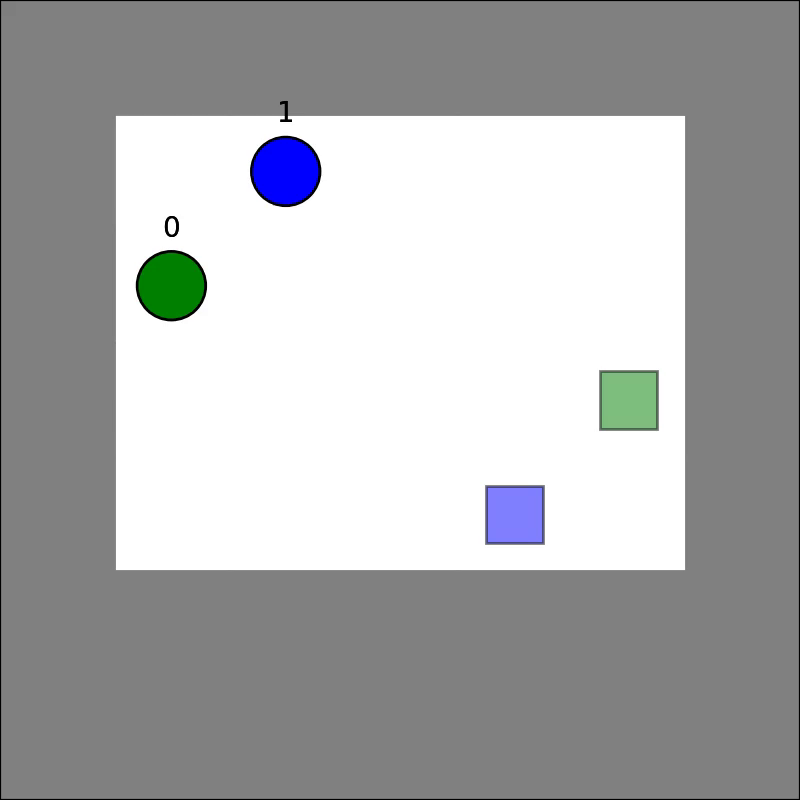
\includegraphics[width=0.3\textwidth]{images/exp4.png}
\end{center}

You can check this by using:

\begin{minted}{bash}
  python run_experiments.py --instance instances/exp4.txt --solver CBS
\end{minted}

If CBS chooses to resolve a vertex collision where agents $a$ and $b$ are both in cell $x$ at time step $t$, then it generates two negative vertex constraints, namely the negative vertex constraint $\langle a,x,t \rangle$ (that prohibits agent $a$ from being in cell $x$ at time step $t$) and the negative vertex constraint $\langle b,x,t \rangle$ (that prohibits agent $b$ from being in cell $x$ at time step $t$). If CBS chooses to resolve an edge collision where agent $a$ moves from cell $x$ to cell $y$ and agent $b$ moves from cell $y$ to cell $x$ at time step $t$, then it generates two negative edge constraints, namely the negative edge constraint $\langle a,x,y,t \rangle$ (that prohibits agent $a$ from moving from cell $x$ to cell $y$ at time step $t$) and the negative edge constraint $\langle b,y,x,t \rangle$ (that prohibits agent $b$ from moving from cell $y$ to cell $x$ at time step $t$). 

CBS with disjoint splitting changes the second constraint in both cases. If CBS with disjoint splitting chooses to resolve a vertex collision, it changes the second negative vertex constraint that prohibits agent $b$ from being in cell $x$ at time step $t$ to a positive vertex constraint that requires agent $a$ to be in cell $x$ at time step $t$. On the other hand, if CBS with disjoint splitting chooses to resolve an edge collision, it changes the second negative edge constraint that prohibits agent $b$ from moving from cell $y$ to cell $x$ at time step $t$ to a positive edge constraint that requires agent $a$ to move from cell $x$ to cell $y$ at time step $t$. In other words, CBS with disjoint splitting changes the second negative constraint (that prohibits the second agent from executing the colliding action) to a positive constraint for the first agent (that requires the first agent to execute the colliding action) in both cases. It could also change the first negative constraint to a positive constraint for the second agent and thus can choose one of the colliding agents freely, for example, randomly.

The reason for this change is that the second constraints are now stronger (meaning more constraining). For example, if an agent $a$ is required to be in cell $x$ at time step $t$, then all other agents (including agent $b$) are automatically prohibited from being in cell $x$ at time step $t$ since they would otherwise collide with agent $a$. Thus, the second positive vertex constraint of CBS with disjoint splitting implicitly includes the second negative vertex constraint of CBS. Thus, CBS with disjoint splitting can be expected to run faster than CBS but remains complete and optimal. More information on CBS with disjoint splitting can be found in \cite{Li19}.

\subsection{Supporting Positive Constraints}

Add code to \texttt{single\_agent\_planner.py} to handle positive vertex and edge constraints (in addition to the current handling of negative vertex and edge constraints). For each constraint dictionary, you should add a new key \texttt{positive} with a binary value that indicates whether the constraint is positive.

\subsection{Converting Collisions to Constraints}

Add code to \texttt{cbs.py} that implements the function \mintinline{python}{disjoint_splitting}. To create a positive constraint, set the item \texttt{positive} in the Python dictionary of the constraint to \mintinline{python}{True}. You can use \mintinline{python}{random.randint(0,1)} to choose one of the two colliding agents randomly.

\subsection{Adjusting the High-Level Search}

Update the code in \texttt{cbs.py} to adjust the high-level search of CBS in the function \mintinline{python}{find_solution} to the new constraints. For each child node, the low level of CBS without disjoint splitting finds a new shortest path for the agent with the newly imposed negative constraint. The paths of the other agents do not need to be updated because they still satisfy the constraints of those agents. However, the low level of CBS with disjoint splitting might have to find new shortest paths not only for the agent with a newly imposed positive constraint but for other agents as well since a positive constraint for an agent implies negative constraints for all other agents. You can compute a list of agent ids of agents that violate a given positive constraint with the helper function \mintinline{python}{paths_violate_constraint}. CBS with disjoint splitting should not add a child node if no path exists for one or more of these agents. Not adding such child nodes is more important for CBS with disjoint splitting than for CBS because there are many more such nodes for CBS with disjoint splitting due to its stronger constraints.

Test your code as before. CBS with disjoint splitting should expand about 8 instead of 11 nodes (although the exact number can vary).

\section{Optional Task 5: Benchmarking MAPF Solvers}

Benchmark your three MAPF solvers on more exciting MAPF instances and compare their performance. You can find benchmark instances at \url{http://mapf.info/index.php/Main/Benchmarks}.

\bibliography{references}
\bibliographystyle{plain}

\end{document}
